% Provenance (never printed): enseignement scientifique premiere (2019),
% theme "La Terre, un astre singulier: la forme de la Terre" (Eratosthenes,
% meridian measurement by triangulation, the metre); see
% sources/book2/PROVENANCE.md. Every length on the ellipsoid is computed in
% figdata/grade-10/meridian_degree.py (WGS 84, ledger wgs84:ellipsoid).
\chapter{قياس الأرض}\label{ch:g10:measuring-the-earth}

قف على شاطئ وراقب سفينة تبتعد نحو عرض البحر. إنها لا تصغر فحسب حتى تتعذر
رؤيتها: بل يختفي هيكلها أولًا، كأنها تغرق، ثم الجزء السفلي من بنيتها العلوية،
ويكون أعلى صاريها آخر ما يختفي. فالبحر بينك وبين السفينة ليس مستويًا، بل
محدّب. وقبل أكثر من اثنين وعشرين قرنًا، حوّل عالم من الإسكندرية ملاحظة
مشابهة --- طول ظل الظهيرة --- إلى قياس لحجم الكوكب كله. ويتتبع هذا الفصل ذلك
القياس وما تلاه من قياسات: سلاسل المثلثات التي مدّها المساحون عبر البلدان،
والبعثات التي أُرسلت إلى المنطقة القطبية الشمالية وإلى خط الاستواء لمعرفة هل
الأرض مفلطحة، وولادة المتر، والأقمار الصناعية التي يُقاس بها الكوكب اليوم.

\begin{omfigure}
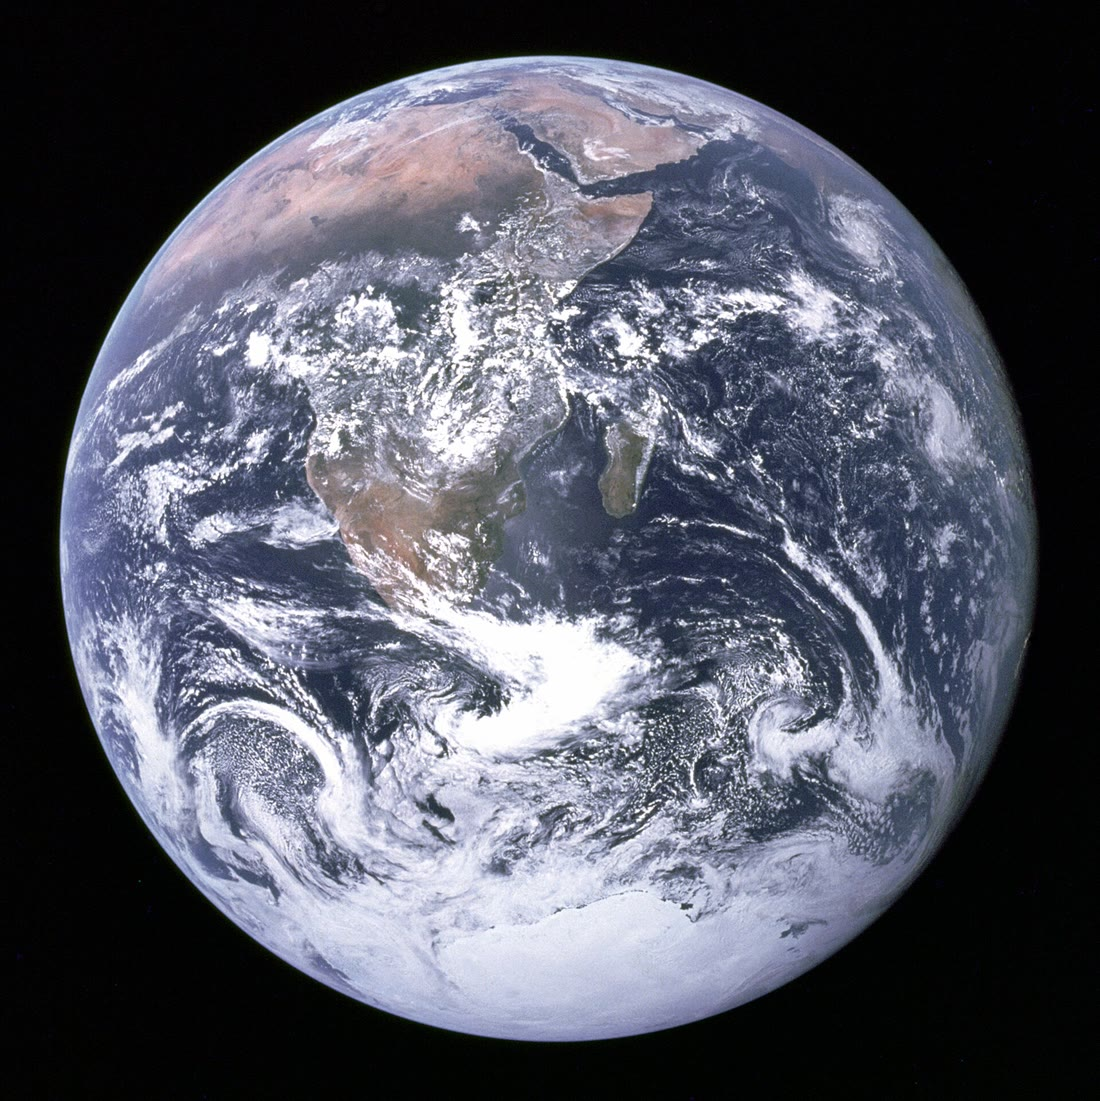
\includegraphics[width=0.5\linewidth]{images/book2/g10-nasa-apollo17-earth.jpg}

{\small الأرض كما صوّرها طاقم أبولو~17 في طريقه إلى القمر، في ديسمبر 1972:
إفريقيا وشبه الجزيرة العربية وجليد القارة القطبية الجنوبية. الصورة: ناسا (ملك
عام).}
\end{omfigure}

\begin{recall}
يُحدَّد موقع مكان على الأرض بعرضه الجغرافي، أي زاويته شمال خط الاستواء أو
جنوبه، وبطوله الجغرافي، أي زاويته شرق خط زوال مرجعي أو غربه؛ وتصل خطوط الزوال
بين القطبين، وتحيط دوائر العرض بالأرض موازيةً لخط الاستواء (الكتاب 1). وفي وسط
متجانس ينتشر الضوء في خطوط مستقيمة، والأشعة التي تبلغ الأرض من الشمس البعيدة
جدًا متوازية (كتب الفيزياء). وفي المثلث القائم، جيب الزاوية الحادة هو الضلع
المقابل مقسومًا على الوتر، وجيب تمامها هو الضلع المجاور مقسومًا على الوتر،
وظلها هو الضلع المقابل مقسومًا على الضلع المجاور (كتب الرياضيات).
\end{recall}

\section{أرض كروية}

قبل أن يتمكن أحد من النظر إلى الأرض من الفضاء بزمن طويل، دلّت ملاحظات عدة على
أنها كروية.
\begin{itemize}
  \item \textbf{سفن وراء الأفق.} السفينة المبتعدة تختفي من أسفلها إلى أعلاها،
        في كل اتجاه وفي كل بحر: فسطح البحر منحنٍ في كل مكان.
  \item \textbf{الظل على القمر.} في أثناء خسوف القمر، يقع ظل الأرض على القمر.
        وحافته دائمًا قوس من دائرة، أيًّا كانت ساعة الليل؛ ولا يُلقي ظلًّا
        مستديرًا في كل اتجاه إلا الكرة.
  \item \textbf{النجوم تتغير مع العرض الجغرافي.} يرى المسافر المتجه شمالًا نجم
        القطب يعلو أكثر فوق الأفق، ونجوم السماء الجنوبية تغيب تحته: فأفق
        المسافر يميل وهو يتحرك على سطح منحنٍ.
  \item \textbf{الدوران حول العالم والنظر من الفضاء.} طافت السفن، ثم
        الطائرات، حول العالم في كل اتجاه؛ ومنذ ستينيات القرن العشرين صُوّر
        الكوكب المستدير كله.
\end{itemize}

\begin{omfigure}
\begin{tikzpicture}[font=\small, >={Stealth[length=2.2mm]}]
  % sea surface: arc of a circle of radius 8 centred at (0,-8) (curvature exaggerated)
  \fill[omDef!10] plot[domain=-4.6:4.6, samples=60] (\x,{sqrt(64-\x*\x)-8}) -- (4.6,-2.2) -- (-4.6,-2.2) -- cycle;
  \draw[omDef!70!black, thick] plot[domain=-4.6:4.6, samples=60] (\x,{sqrt(64-\x*\x)-8});
  % observer on a small tower at x=-4 (surface y=-1.072), eye at y=-0.235
  \draw[black!70, line width=1pt] (-4,-1.072) -- (-4,-0.235);
  \fill (-4,-0.235) circle (2pt);
  \node[anchor=east, align=right] at (-4.1,-0.2) {عين\\الراصد};
  % line of sight tangent at x=-0.5 (y=-0.0156, slope 0.0626)
  \draw[omThm!80!black, thick] (-4,-0.235) -- (4.4,0.290);
  \node[omThm!80!black, anchor=south, rotate=3.6] at (1.3,0.1) {خط النظر};
  \fill[omThm!80!black] (-0.5,-0.0156) circle (1.4pt);
  % ship at x=3 (surface y=-0.584), tilted 22 degrees with the local vertical
  \begin{scope}[shift={(3,-0.584)}, rotate=-22]
    \fill[black!12] (-0.6,0) -- (0.6,0) -- (0.75,0.32) -- (-0.75,0.32) -- cycle;
    \draw[black!45, densely dashed] (-0.6,0) -- (0.6,0) -- (0.75,0.32) -- (-0.75,0.32) -- cycle;
    \draw[black!45, densely dashed] (0,0.32) -- (0,0.95);
    \draw[black!80, line width=1pt] (0,0.95) -- (0,1.55);
    \fill[black!80] (0,1.55) -- (0.32,1.25) -- (0,1.25) -- cycle;
  \end{scope}
  \node[anchor=north, align=center, font=\footnotesize] at (2.9,-1.25) {الهيكل وأسفل الصاري\\يحجبهما التحدب};
  \node[anchor=north, font=\footnotesize] at (-0.5,-0.1) {الأفق};
\end{tikzpicture}

{\small لماذا تختفي السفينة من أسفلها إلى أعلاها: لا يرى الراصد إلا ما يقع فوق
خط النظر الذي يلامس البحر عند الأفق. وقد بولغ كثيرًا في تصوير
الانحناء.}
\end{omfigure}

\section{إراتوستينس يقيس الأرض}

كان إراتوستينس القوريني (276--194 ق.م.) أمين مكتبة الإسكندرية. وقد بلغه أن
الشمس في سيين، أي أسوان الحالية، في أعالي النيل، تضيء قاع بئر كله عند الظهيرة
في يوم الانقلاب الصيفي: فقد كانت عندئذ عمودية تمامًا فوق الرأس. وفي الإسكندرية،
في اللحظة نفسها، كان لعمود رأسي ظل قصير: إذ كانت أشعة الشمس تصنع مع الرأسي
زاوية تقارب \qty{7.2}{\degree}، أي جزءًا من خمسين من الدائرة الكاملة.
% ledger: erat:method, erat:stadion

\begin{omfigure}
\begin{tikzpicture}[font=\small, >={Stealth[length=2.2mm]}]
  \def\R{2.4}
  \fill[omDef!8] (0,0) circle (\R);
  \draw[omDef!70!black, thick] (0,0) circle (\R);
  \coordinate (O) at (0,0);
  \coordinate (S) at (\R,0);
  \coordinate (A) at ({\R*cos(25)},{\R*sin(25)});
  \coordinate (T) at ({(\R+0.75)*cos(25)},{(\R+0.75)*sin(25)});
  \coordinate (T2) at ({(\R+1.75)*cos(25)},{(\R+1.75)*sin(25)});
  % radii
  \draw[black!70] (O) -- (S);
  \draw[black!70] (O) -- (A);
  \draw[black!40, densely dashed] (A) -- (T2);
  \fill (O) circle (1.5pt) node[below left] {المركز};
  % stick at Alexandria, along the radius
  \draw[line width=1.6pt, black!85] (A) -- ($(A)!0.6!(T)$);
  % well at Syene
  \draw[black!80, thick] ({\R-0.38},-0.12) -- (\R,-0.12) ($(S)+(0,0.12)$) -- ({\R-0.38},0.12);
  % parallel sun rays coming from the right
  \foreach \y in {-1.6,-0.8,0.8,1.6} \draw[->, omThm!70, thick] (6.6,\y) -- (4.4,\y);
  \draw[->, omThm!85!black, thick] (6.6,0) -- (\R+0.05,0);
  \draw[->, omThm!85!black, thick] (6.6,{(\R+0.45)*sin(25)}) -- ({(\R+0.45)*cos(25)+0.03},{(\R+0.45)*sin(25)});
  \node[omThm!85!black, align=center, anchor=west] at (4.6,2.35) {\foreignlanguage{arabic}{ضوء الشمس:}\\أشعة متوازية};
  % angles
  \draw[omExo!80!black, thick] (0.75,0) arc (0:25:0.75);
  \node[omExo!80!black] at (1.05,0.22) {$\alpha$};
  \coordinate (Q) at ($(A)!0.6!(T)$);
  \draw[omExo!80!black, thick] ($(Q)+(0.8,0)$) arc (0:25:0.8);
  \node[omExo!80!black] at ($(Q)+({1.08*cos(12.5)},{1.08*sin(12.5)})$) {$\alpha$};
  \node[anchor=east] at ($(A)+(-0.12,0.18)$) {الإسكندرية};
  \node[anchor=north west] at ($(S)+(0.3,-0.12)$) {سيين};
  \node[font=\footnotesize, anchor=north] at ($(O)!0.5!(S)+(0.2,-0.05)$) {};
  \draw[<->, black!60] ({(\R-0.3)*cos(3)},{(\R-0.3)*sin(3)}) arc (3:22:{\R-0.3});
  \node[anchor=east, font=\footnotesize] at ({(\R-0.35)*cos(13)},{(\R-0.35)*sin(13)}) {$d$};
\end{tikzpicture}

{\small استدلال إراتوستينس. في سيين تكون الشمس فوق الرأس تمامًا: فأشعتها تتجه
نحو مركز الأرض. وفي الإسكندرية يصنع عمود رأسي، يتجه هو أيضًا نحو المركز،
زاوية $\alpha$ مع الأشعة. والزاوية عند المركز بين المكانين هي الزاوية $\alpha$
نفسها. وقد بولغ في الزاوية: فهي لم تكن إلا
\qty{7.2}{\degree}.}
\end{omfigure}

\begin{proposition}[علاقة إراتوستينس]\label{prop:g10:measuring-the-earth:eratosthenes}
إذا وقع مكانان على خط الزوال نفسه، تفصل بينهما مسافة $d$، وكانت أشعة الشمس عند
الظهيرة تصنع مع الرأسي زاويتين تختلفان بمقدار $\alpha$ (بالدرجات)، فإن محيط
الأرض هو
\[
  C = \frac{\qty{360}{\degree}}{\alpha}\, d .
\]
\end{proposition}

\begin{proof}
الشمس بعيدة جدًا حتى إن أشعتها التي تبلغ المكانين متوازية. وفي كل مكان يتجه
الرأسي نحو مركز الأرض. وفي الشكل، الشعاع الذي يبلغ العمود ونصف القطر المار
بسيين مستقيمان متوازيان، ونصف القطر المار بالإسكندرية يقطعهما كليهما: فالزاوية
$\alpha$ بين العمود والشعاع والزاوية عند المركز بين نصفي القطر زاويتان متبادلتان
داخليًا، فهما متساويتان. والقوس $d$ هو الكسر نفسه من المحيط الكامل الذي تمثله
الزاوية $\alpha$ من الدورة الكاملة:
$d/C = \alpha/\qty{360}{\degree}$.
\end{proof}

\begin{method}[قياس محيط من ظلّين]\label{met:g10:measuring-the-earth:shadows}
\begin{enumerate}
  \item اختر مكانين على خط الزوال نفسه (أو قريبًا منه) وقِس المسافة
        $d$ بينهما في اتجاه الشمال--الجنوب.
  \item عند الظهيرة المحلية من اليوم نفسه، قِس في كل مكان الزاوية بين عمود
        رأسي وأشعة الشمس: $\tan \theta = s/h$، حيث $h$ ارتفاع العمود و$s$ طول
        ظله. لا تنظر أبدًا إلى الشمس نفسها: فالزاوية تُقرأ من الظل
        وحده.
  \item خذ الفرق $\alpha$ بين الزاويتين وطبّق
        $C = (360/\alpha)\,d$.
\end{enumerate}
\end{method}

\begin{example}[أعداد إراتوستينس]\label{ex:g10:measuring-the-earth:numbers}
% ledger: erat:method, erat:stadion
اعتمد إراتوستينس للمسافة من الإسكندرية إلى سيين 5000
\emph{ستاديون}، وهي وحدة طول يونانية. ومع $\alpha = 1/50$ من الدائرة،
\[
  C = 50 \times 5000 = 250\,000 \text{ ستاديون}.
\]
فكم كان طول الستاديون؟ ما زال المؤرخون يختلفون في ذلك. فإذا كان
\qty{157.2}{m} كان $C \approx \qty{39300}{km}$؛ وإذا كان \qty{166.7}{m} كان
$C \approx \qty{41700}{km}$. أما المحيط الحقيقي لخط الزوال فهو
\qty{40008}{km}: وفي الحالتين لم يبتعد إراتوستينس إلا ببضعة في المئة.
\end{example}

\begin{remark}[ما افتُرض]\label{rem:g10:measuring-the-earth:assumptions}
افترض إراتوستينس أن الأرض كروية، وأن الشمس بعيدة بما يكفي لتكون أشعتها
متوازية، وأن سيين تقع على المدار تمامًا (حيث يمكن أن تكون الشمس فوق الرأس)، وأن
سيين تقع جنوب الإسكندرية تمامًا. وكان كل ذلك صحيحًا تقريبًا لا تمامًا: فأسوان
تقع شرق الإسكندرية بنحو \qty{3}{\degree} من الطول الجغرافي. والمهم هو مركّبة
المسافة في اتجاه الشمال--الجنوب، أي المركّبة على طول خط الزوال.
% ledger: geonames:aswan, geonames:alexandria
\end{remark}

\section{التثليث}

قياس مسافة طويلة على الأرض بسلسلة أو بقضيب عمل بطيء، وهو عبر الأنهار والغابات
والجبال مستحيل. أما الزوايا فيمكن قياسها بدقة كبيرة بمنظار مثبت على دائرة
مدرّجة، يُوجَّه تباعًا نحو إشارتين بعيدتين. ومنذ القرن الثامن عشر استعمل
المساحون ذلك لقياس بلدان بأكملها.

\begin{definition}[الجيوديسيا]\label{def:g10:measuring-the-earth:geodesy}
\emph{الجيوديسيا}\index{جيوديسيا} علم يقيس شكل الأرض وحجمها ومواقع النقاط
على سطحها، ويتابع تغيرها مع الزمن.
\end{definition}

\begin{definition}[التثليث]\label{def:g10:measuring-the-earth:triangulation}
\emph{التثليث}\index{تثليث} طريقة تحدد مواقع نقاط بعيدة بسلسلة من المثلثات:
يُقاس ضلع واحد، هو \emph{خط القاعدة}، على الأرض بعناية كبيرة؛ وتُقاس كل زوايا
المثلثات من رؤوسها؛ ثم تُحسب كل الأضلاع
الأخرى.
\end{definition}

يستند الحساب إلى علاقة واحدة بين أضلاع أي مثلث وزواياه. في مثلث $ABC$، نرمز
بالرموز $a$ و$b$ و$c$ إلى الأضلاع المقابلة للرؤوس $A$ و$B$ و$C$، ونرمز
بالرموز $A$ و$B$ و$C$ أيضًا إلى الزوايا عند هذه الرؤوس.

\begin{proposition}[قانون الجيوب]\label{prop:g10:measuring-the-earth:sine-rule}
في أي مثلث $ABC$،
\[
  \frac{a}{\sin A} = \frac{b}{\sin B} = \frac{c}{\sin C}.
\]
\end{proposition}

\begin{proof}
ارسم الارتفاع النازل من $C$، الذي يلاقي المستقيم $AB$ في $H$ (اللوحة الثانية
من الشكل أدناه)؛ ولنكتب $h = CH$. في المثلث القائم $AHC$، $\sin A = h/b$،
إذن $h = b \sin A$. وفي المثلث القائم $BHC$، $\sin B = h/a$، إذن
$h = a \sin B$. ومنه $b \sin A = a \sin B$، أي $a/\sin A = b/\sin B$.
(وإذا كانت الزاوية عند $B$ منفرجة، وقعت $H$ وراء $B$ وكانت زاوية المثلث
القائم عند $B$ هي $\qty{180}{\degree} - B$، ولها الجيب نفسه.) والاستدلال نفسه
مع الارتفاع النازل من $A$ يعطي $b/\sin B = c/\sin C$.
\end{proof}

\begin{omfigure}
\begin{tikzpicture}[font=\small, >={Stealth[length=2mm]}]
  \begin{scope}
    \coordinate (A) at (0,0); \coordinate (B) at (2.0,0.25);
    \coordinate (C) at (0.9,1.9); \coordinate (D) at (3.0,2.1);
    \coordinate (E) at (1.9,3.8); \coordinate (F) at (3.9,4.1);
    \coordinate (G) at (2.7,5.6);
    \draw[black!60] (A) -- (C) -- (B) (C) -- (D) -- (B) (C) -- (E) -- (D) -- (F) -- (E) -- (G) -- (F);
    \draw[omThm!85!black, line width=2pt] (A) -- (B);
    \foreach \p in {A,B,C,D,E,F,G} \fill (\p) circle (1.6pt);
    \node[below left] at (A) {$A$}; \node[below right] at (B) {$B$};
    \node[left] at (C) {$C$}; \node[right] at (D) {$D$};
    \node[left] at (E) {$E$}; \node[right] at (F) {$F$}; \node[above] at (G) {$G$};
    \node[omThm!85!black, anchor=north, font=\footnotesize] at (1.25,-0.3) {خط القاعدة المقيس};
    \draw[omExo!80!black] ($(A)!0.28!(B)$) arc[start angle=7, end angle=64.6, radius=0.56];
    \draw[omExo!80!black] ($(B)!0.3!(A)$) arc[start angle=187, end angle=123, radius=0.6];
    \draw[black!50, densely dashed] (-0.5,0) -- (-0.5,5.6);
    \draw[->, black!70] (-0.5,5.0) -- (-0.5,5.8) node[above] {ش};
    \node[rotate=90, font=\footnotesize, black!60, anchor=south] at (-0.5,2.6) {خط الزوال};
  \end{scope}
  \begin{scope}[xshift=6.2cm, yshift=0.6cm]
    \coordinate (A) at (0,0); \coordinate (B) at (4,0); \coordinate (C) at (1.4,2.6);
    \coordinate (H) at (1.4,0);
    \draw[thick] (A) -- (B) -- (C) -- cycle;
    \draw[omDef!80!black, densely dashed] (C) -- (H);
    \draw[omDef!80!black] (1.4,0.22) -- (1.62,0.22) -- (1.62,0);
    \node[below left] at (A) {$A$}; \node[below right] at (B) {$B$};
    \node[above] at (C) {$C$}; \node[below] at (H) {$H$};
    \node[omDef!80!black, anchor=west] at (1.4,1.05) {$h$};
    \node[anchor=south east] at (0.7,1.3) {$b$};
    \node[anchor=south west] at (2.75,1.35) {$a$};
    \node[anchor=north] at (2.7,-0.02) {$c$};
    \draw[omExo!80!black] (0.5,0) arc (0:61.7:0.5);
    \draw[omExo!80!black] (3.45,0) arc (180:135:0.55);
  \end{scope}
\end{tikzpicture}

{\small في اليسار: سلسلة مثلثات ممتدة على طول خط زوال انطلاقًا من خط قاعدة مقيس
$AB$؛ ويشير القوسان إلى اثنتين من الزوايا الكثيرة التي قيست بالأداة. وفي
اليمين: الارتفاع $h$ النازل من $C$، مكتوبًا بطريقتين، يعطي قانون
الجيوب.}
\end{omfigure}

\begin{method}[حساب سلسلة تثليث]\label{met:g10:measuring-the-earth:chain}
\begin{enumerate}
  \item في المثلث الأول $ABC$، يُقاس خط القاعدة $c = AB$ والزاويتان عند
        $A$ و$B$؛ والزاوية الثالثة هي
        $C = \qty{180}{\degree} - A - B$ (وقياسها يتحقق من
        الزاويتين الأخريين).
  \item يعطي قانون الجيوب الضلعين الآخرين:
        $b = AC = c \sin B / \sin C$ و$a = BC = c \sin A / \sin C$.
  \item يصبح الضلع المحسوب الضلعَ المعلوم في المثلث التالي، وهكذا
        على طول السلسلة.
  \item وأخيرًا، تُحسب مركّبة كل ضلع في اتجاه الشمال--الجنوب بجيب تمام زاويته
        مع خط الزوال، ثم تُجمع المركّبات.
\end{enumerate}
\end{method}

\begin{example}[مثلث واحد]\label{ex:g10:measuring-the-earth:triangle}
يُقاس خط قاعدة $AB = \qty{8.000}{km}$؛ ومن $A$ تُرى الإشارة $C$ على زاوية
\qty{70}{\degree} من اتجاه $B$، ومن $B$ على زاوية
\qty{60}{\degree} من اتجاه $A$. إذن $C = \qty{50}{\degree}$، ومن ثم
\[
  AC = \frac{8.000 \times \sin 60^\circ}{\sin 50^\circ} = \frac{8.000 \times 0.8660}{0.7660}
  \approx \qty{9.044}{km}, \qquad
  BC = \frac{8.000 \times \sin 70^\circ}{\sin 50^\circ} \approx \qty{9.814}{km}.
\]
لم تُقطع مشيًا أي مسافة غير خط القاعدة.
\end{example}

\begin{example}[خط زوال المتر]\label{ex:g10:measuring-the-earth:meridian}
% ledger: metre:1791, metre:survey, geonames:dunkirk, geonames:barcelona (arc computed in figdata/grade-10/meridian_degree.py)
في مارس 1791 عُرّف المتر بأنه جزء من عشرة ملايين من المسافة بين القطب وخط
الاستواء على طول خط زوال. ولإيجاد تلك المسافة، قاس فلكيان، هما جان باتيست
ديلامبر وبيير ميشان، \omterm{def:g10:measuring-the-earth:triangulation}{بالتثليث} قوس خط الزوال من دنكرك، على بحر الشمال، إلى
برشلونة، على البحر المتوسط --- في عمل استغرق قرابة سبع سنين، تولى فيه ديلامبر
الثلثين الشماليين، وميشان الثلث الجنوبي. ويختلف عرضا المدينتين بمقدار
\qty{9.646}{\degree}؛ وعلى الإهليلجي الحديث يبلغ طول القوس بين دائرتي عرضهما
\qty{1072.2}{km}. ومعرفة طول قوس وفرق العرض بين طرفيه تعطي طول الدرجة الواحدة؛
ثم يعطي شكل الأرض ربع خط الزوال كله. وصُنعت مقاييس بلاتينية للمتر الجديد
عام 1799 وحُفظت في الأرشيف الوطني.
\end{example}

\begin{history}[الدائرة المكرِّرة]
قيست زوايا خط زوال المتر \emph{بالدائرة
المكرِّرة}، وهي أداة صنعها جان شارل دو بوردا: منظاران على دائرة مدرّجة،
يوجَّهان بالتناوب نحو إشارتين مرات كثيرة، فتنقسم أخطاء قراءة التدريج على عدد
مرات التكرار.
\begin{center}
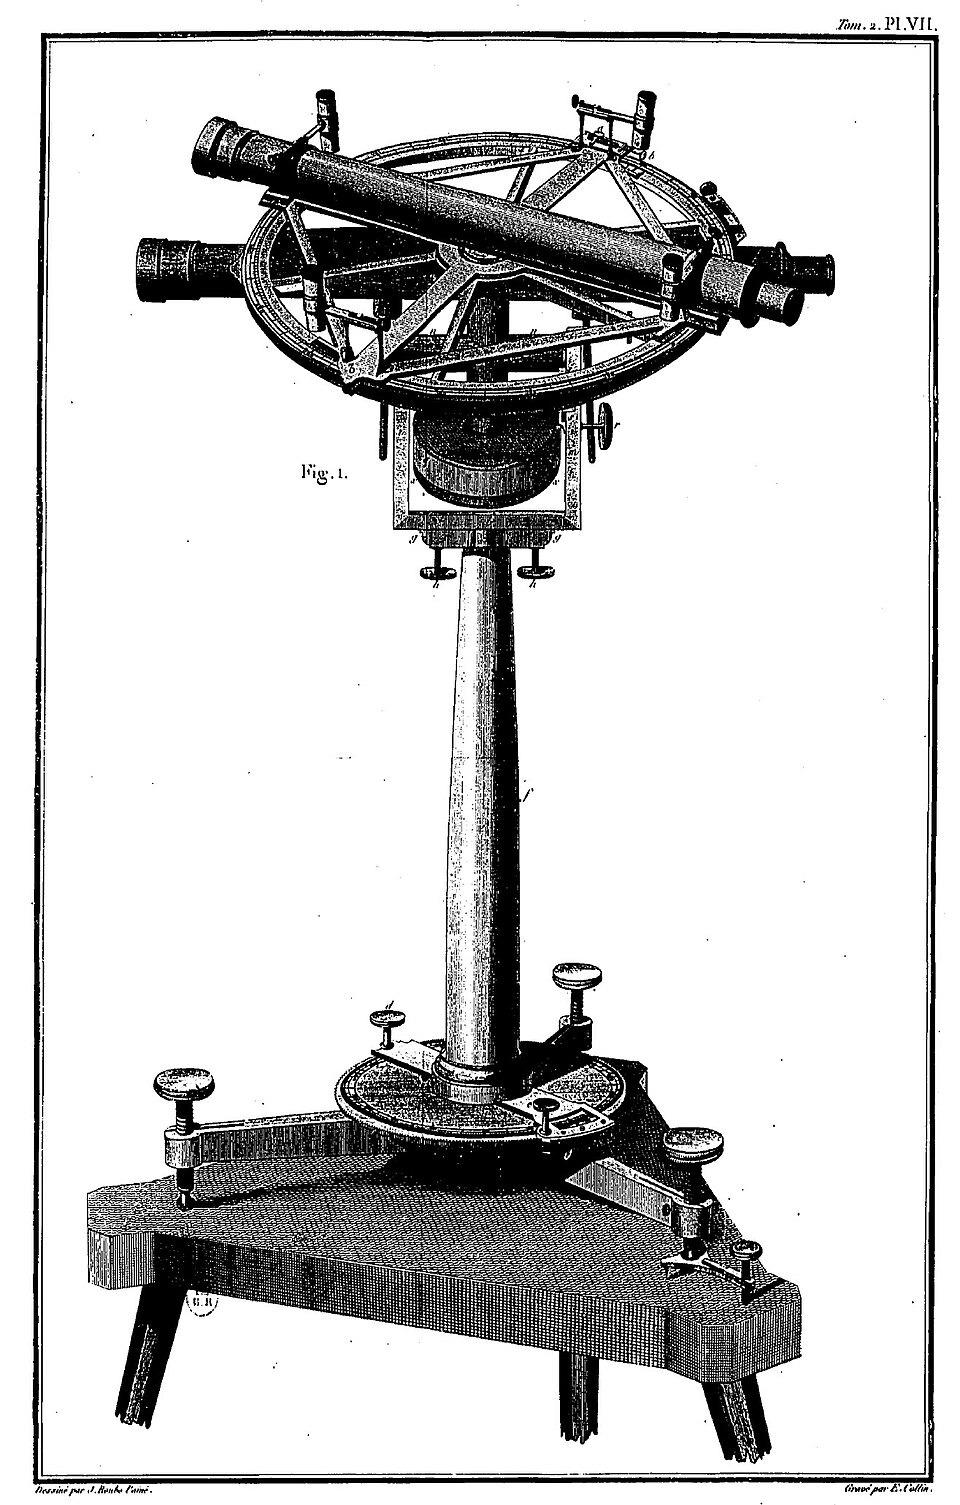
\includegraphics[width=0.3\linewidth]{images/book2/g10-delambre-repeating-circle.jpg}

{\small دائرة مكرِّرة منصوبة لقياس الزوايا الأفقية، كما نُقشت في تقرير
ديلامبر عن القياس (1807). ملك عام (ويكيميديا
كومنز).}
\end{center}
\end{history}

\section{أرض مفلطحة}

نحو عام 1687، استنتج إسحاق نيوتن من نظريته في الجاذبية أن الأرض الدوّارة لا بد
أن تكون مجسمًا مفلطحًا عند القطبين منتفخًا عند خط الاستواء. لكن قياسات درجات
خط الزوال التي أجراها فلكيو مرصد باريس بدت تقول العكس: أرضًا مستطيلة عند
القطبين. وحُسمت المسألة بقياس طول درجة واحدة من العرض الجغرافي في مكانين
متباعدين قدر الإمكان.
% ledger: figure:expeditions

\begin{omfigure}
\begin{tikzpicture}[font=\small, >={Stealth[length=2mm]}]
  \def\a{3.0} \def\b{2.3}
  \draw[black!35, densely dashed] (0,0) circle (\a);
  \fill[omDef!8] (0,0) ellipse ({\a} and {\b});
  \draw[omDef!70!black, thick] (0,0) ellipse ({\a} and {\b});
  \draw[black!50] (-3.4,0) -- (3.7,0);
  \draw[black!50] (0,-2.6) -- (0,3.3);
  \draw[<->, omThm!85!black] (0,-0.3) -- (\a,-0.3);
  \node[omThm!85!black, below] at (1.5,-0.3) {$a$};
  \draw[<->, omThm!85!black] (-0.3,0) -- (-0.3,\b);
  \node[omThm!85!black, left] at (-0.3,1.15) {$b$};
  \node[above right] at (0,\b) {ش};
  \node[anchor=south east] at (3.0,-2.5) {};
  \node[anchor=west] at (3.7,0) {خط الاستواء};
  % normal at t = 45 deg: P = (2.121, 1.626); crosses the equator at (0.874,0), the axis at (0,-1.14)
  \coordinate (P) at (2.121,1.626);
  \draw[omExo!85!black, thick] (P) -- ($(P)!1.35!(0.874,0)$);
  \draw[omExo!85!black, thick, ->] (P) -- ($(P)!-0.45!(0.874,0)$);
  \fill (P) circle (1.6pt);
  \node[anchor=west, align=left, font=\footnotesize] at (2.85,2.35) {الرأسي المحلي\\(خيط الشاقول)};
  \draw[omExo!85!black] (1.45,0) arc (0:52.5:0.58);
  \node[omExo!85!black] at (1.62,0.32) {$\varphi$};
  \fill (0,0) circle (1.3pt);
  \node[anchor=north east, font=\footnotesize] at (0,0) {المركز};
  \node[black!50, font=\footnotesize, anchor=south] at (-2.2,2.15) {كرة};
\end{tikzpicture}

{\small أرض مفلطحة، مع مبالغة كبيرة في \omterm{def:g10:measuring-the-earth:ellipsoid}{التفلطح} (\omterm{def:g10:measuring-the-earth:ellipsoid}{فالتفلطح} الحقيقي أصغر من أن
يُرى بهذا المقياس). الرأسي في مكان ما عمودي على السطح؛ ولا يتجه تمامًا نحو
المركز. والعرض الجغرافي $\varphi$ للمكان هو الزاوية بين رأسيّه ومستوي خط
الاستواء.}
\end{omfigure}

يُقاس العرض الجغرافي من النجوم: فهو الزاوية بين الرأسي المحلي ومستوي خط
الاستواء. وعلى أرض مفلطحة يكون السطح قرب القطبين أقل انحناءً منه قرب خط الاستواء.
وحيث يكون السطح أقل انحناءً، يجب أن يُقطع عليه مسافة أطول كي يدور الرأسي درجة
واحدة: \emph{فدرجة العرض أطول قرب القطبين}.

\begin{history}[لابلاند والبيرو]
% ledger: figure:expeditions, figure:degrees
في عام 1735 أرسلت أكاديمية العلوم في باريس بعثة إلى خط الاستواء، في ولاية
البيرو الإسبانية (الإكوادور اليوم)؛ وعملت هناك تسع سنين، حتى 1744. وفي
1736--1737 قاست بعثة ثانية، بقيادة بيير لوي مورو دو موبرتوي ومعه الرياضي
الشاب ألكسيس كليرو، درجة من خط الزوال في لابلاند، قرب الدائرة القطبية الشمالية.
فجاءت درجة لابلاند \num{57437} \emph{توازًا} (وحدة الطول القديمة؛ نحو
\qty{111.95}{km})، ودرجة البيرو \num{56737} توازًا فقط: فالدرجة أطول قرب القطب،
وكان نيوتن على حق. وكان العددان يقتضيان تفلطحًا يقارب $1/205$ --- وهو كبير
أكثر مما ينبغي، كما أظهرت المسوح اللاحقة، لكن مسألة الإشارة حُسمت.
\end{history}

\begin{omfigure}
\begin{tikzpicture}
\begin{axis}[omrecord, width=0.82\linewidth, height=5.4cm, xmin=0, xmax=90,
  ymin=110.45, ymax=111.8, xlabel={\foreignlanguage{arabic}{العرض الجغرافي \babelsublr{(\unit{\degree})}}},
  ylabel={\foreignlanguage{arabic}{طول \babelsublr{\qty{1}{\degree}} من العرض \babelsublr{(km)}}}, xtick={0,15,...,90},
  ytick={110.6,110.8,...,111.8}, yticklabel style={/pgf/number format/fixed, /pgf/number format/fixed zerofill, /pgf/number format/precision=1}]
\addplot[omDef!85!black, line width=1.1pt] table[x=lat_deg, y=deg_km] {figdata/out/grade-10-meridian_degree.dat};
\addplot[only marks, mark=*, mark size=1.8pt, omThm!85!black] coordinates {(0,110.574) (45,111.132) (66,111.507) (90,111.694)};
\node[anchor=south west, font=\footnotesize] at (axis cs:2,110.6) {110.57 km};
\node[anchor=north east, font=\footnotesize] at (axis cs:89,111.56) {111.69 km};
\node[anchor=north west, font=\footnotesize] at (axis cs:46,111.12) {111.13 km};
\node[anchor=south east, font=\footnotesize] at (axis cs:65,111.53) {\foreignlanguage{arabic}{\babelsublr{111.51 km} عند \babelsublr{\ang{66}}، في لابلاند}};
\end{axis}
\end{tikzpicture}

{\small طول درجة واحدة من العرض على \omterm{def:g10:measuring-the-earth:ellipsoid}{الإهليلجي المرجعي} في
\cref{def:g10:measuring-the-earth:ellipsoid}، من خط الاستواء إلى القطب.
محسوب من إهليلجي WGS~84.}
\end{omfigure}

\begin{definition}[الإهليلجي المرجعي والتفلطح]\label{def:g10:measuring-the-earth:ellipsoid}
\emph{الإهليلجي المرجعي}\index{إهليلجي مرجعي} سطح يُحصل عليه بتدوير قطع ناقص
حول محوره الأصغر، ويُختار ليطابق شكل الأرض بأقرب ما يمكن. ويُسمّى
\emph{نصف قطره الاستوائي} $a$، و\emph{نصف قطره القطبي} $b$، أما
\emph{تفلطحه}\index{تفلطح} فهو
\[
  f = \frac{a-b}{a}.
\]
\end{definition}

\begin{proposition}[أبعاد الأرض]\label{prop:g10:measuring-the-earth:dimensions}
% ledger: wgs84:ellipsoid, earth:Req, earth:Rpol, earth:Rmean (lengths computed in figdata/grade-10/meridian_degree.py)
\omterm{def:g10:measuring-the-earth:ellipsoid}{للإهليلجي المرجعي} الذي تستعمله أنظمة التحديد بالأقمار الصناعية (WGS~84)
\[
  a = \qty{6378.137}{km}, \qquad b = \qty{6356.752}{km}, \qquad
  f = \frac{1}{298.257}.
\]
فنصف القطر القطبي أقصر من نصف القطر الاستوائي بمقدار \qty{21.4}{km}. وطول خط
الاستواء \qty{40075}{km}، وطول خط الزوال، من قطب إلى قطب ذهابًا وإيابًا،
\qty{40008}{km}؛ أما ربع خط الزوال، من خط الاستواء إلى أحد القطبين، فطوله
\qty{10001.966}{km}. وطول درجة العرض الواحدة \qty{110.574}{km} عند خط
الاستواء و\qty{111.694}{km} عند القطبين. أما درجة الطول فطولها
\qty{111.32}{km} على خط الاستواء، وتقصر نحو القطبين بما يقارب
$\cos \varphi$.
\end{proposition}

\begin{example}[درجة من الطول الجغرافي]\label{ex:g10:measuring-the-earth:longitude}
دائرة العرض عند العرض $\varphi$ دائرة نصف قطرها هو بعدها عن المحور، أي نحو
$R \cos \varphi$. وعند \qty{60}{\degree} ش يبلغ محيطها نحو نصف محيط خط الاستواء،
وتبلغ درجة الطول نحو $111.32 \times \cos 60^\circ \approx \qty{55.7}{km}$ (ويعطي
الإهليلجي \qty{55.80}{km}).
\end{example}

\begin{remark}[ما مدى كروية الأرض؟]\label{rem:g10:measuring-the-earth:round}
\omterm{def:g10:measuring-the-earth:ellipsoid}{التفلطح} $1/298$ صغير. فعلى مجسم كرة أرضية قطره \qty{30}{cm}، لا يقصر القطر
القطبي عن القطر الاستوائي إلا بمقدار \qty{1}{mm} --- وهذا غير مرئي. وأعمق خندق
محيطي، الذي يبلغ نحو \qty{11}{km} تحت مستوى سطح البحر، يصبح خدشًا عمقه نحو ربع
مليمتر. ففي معظم الأغراض تكون الأرض كرة نصف قطرها المتوسط \qty{6371}{km}؛ أما
للمواقع الدقيقة، فلا بد من الإهليلجي.
% ledger: earth:Rmean, usgs:trench-depth
\end{remark}

\section{الجيوديسيا اليوم}

\begin{omfigure}
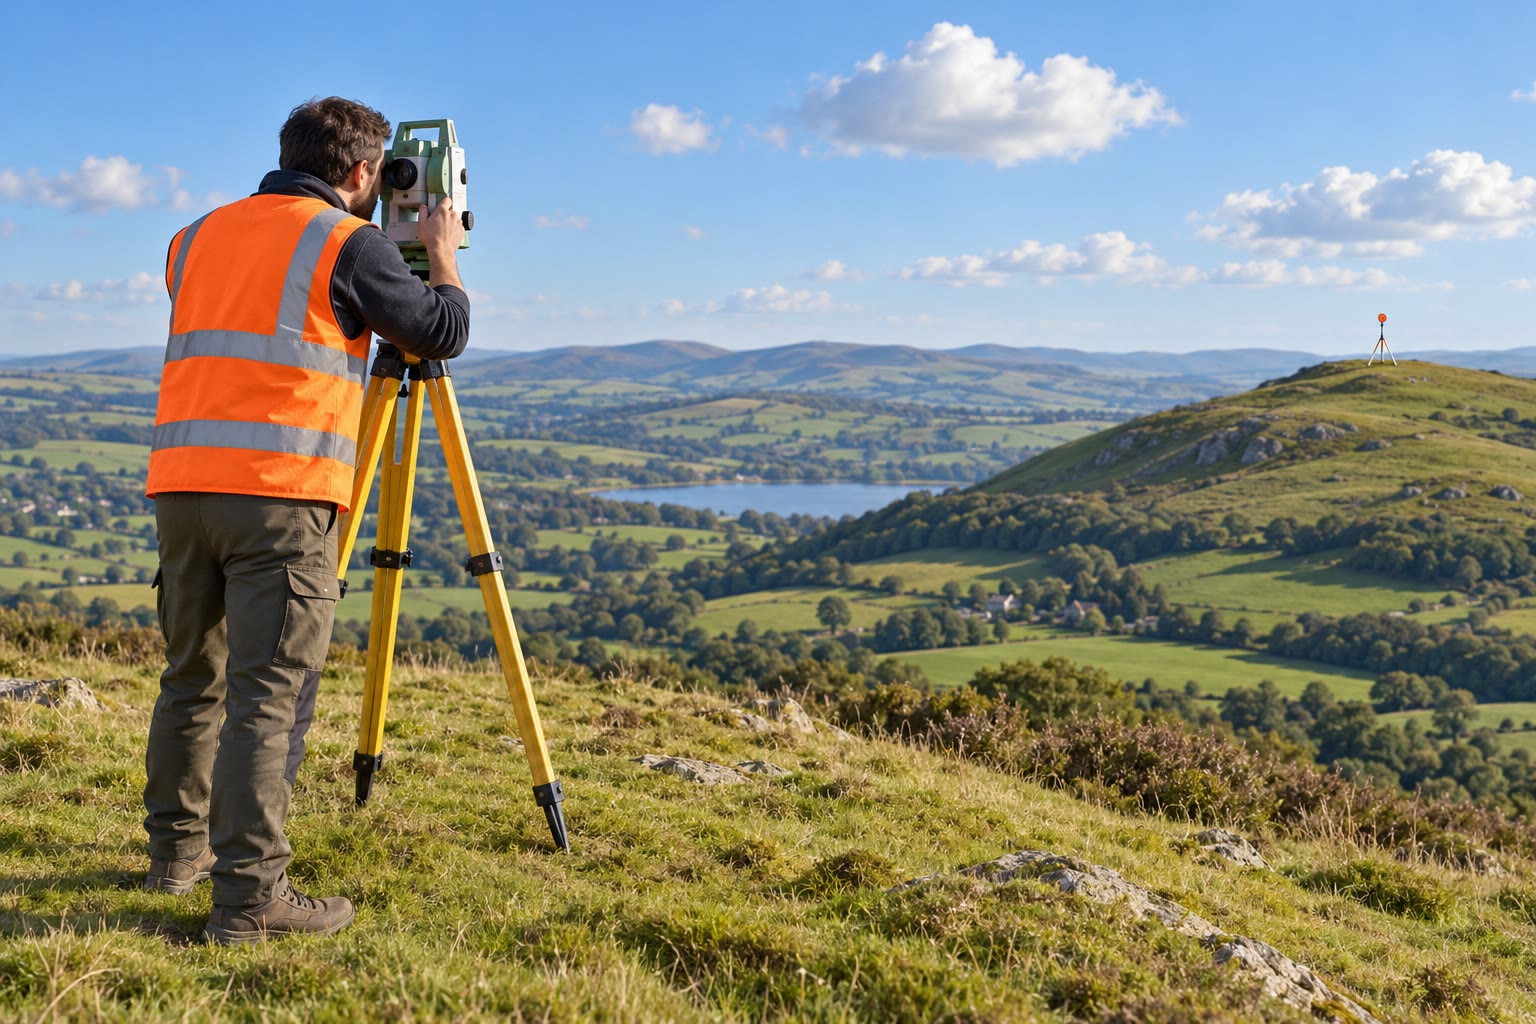
\includegraphics[width=0.7\linewidth]{images/book2/ai/g10-surveyor-theodolite.jpg}

{\small مسّاح في أثناء عمله بأداة حديثة تقيس الزوايا، وتقيس المسافات أيضًا
بحزمة من الضوء؛ وتنتصب إشارة مساحة على التلة
البعيدة.}
\end{omfigure}

حلّت الأقمار الصناعية محل التثليثات الكبرى في القرنين الثامن عشر والتاسع عشر.
فجهاز استقبال على الأرض يلتقط إشارات أقمار صناعية عدة مواقعها معلومة في كل
لحظة، ويحسب موقعه هو من أزمنة انتقال الإشارات (الكتاب 1). وتقيس شبكات من
أجهزة الاستقبال الدائمة، المثبتة في الصخر الأساسي في أنحاء العالم كله، مواقعها
باستمرار. وهي تحدد الإطار المرجعي الذي تُعطى فيه كل خريطة وكل موقع بالأقمار
الصناعية، وهي تتحرك: فتُظهر صفائح الغلاف الصخري تنجرف ببضعة سنتيمترات في
السنة
(\cref{ch:g11:plate-motions}).
% ledger: usgs:gps

\begin{inthefield}[قياس الأرض اليوم]
يثبّت علماء \omterm{def:g10:measuring-the-earth:geodesy}{الجيوديسيا} هوائيات على أعمدة خرسانية مغروسة في الصخر الأساسي،
بعيدًا عن المباني والأشجار، ويسجلون مواقعها كل بضع ثوانٍ طوال سنوات. ويجمعون
هذه القياسات مع قياسات من تلسكوبات راديوية ترصد مجرات بعيدة جدًا، ومع حزم ليزر
تُطلق نحو أقمار صناعية تحمل مرايا. وما زال المساحون في مواقع البناء وفي الريف
يقيسون الزوايا والمسافات بأدوات على حوامل ثلاثية، ويربطونها بإطار الأقمار
الصناعية.
\end{inthefield}

\section{تمارين}

\begin{exercise}[$\star$]\label{exo:g10:measuring-the-earth:1}
اذكر ثلاث ملاحظات ممكنة دون مغادرة سطح الأرض تدل على أن الأرض كروية. وفسّر
لكل منها، في جملة واحدة، لماذا لا يمكن أن تنتج عن أرض
مسطحة.
\end{exercise}

\begin{exercise}[$\star$]\label{exo:g10:measuring-the-earth:2}
ما \omterm{def:g10:measuring-the-earth:geodesy}{الجيوديسيا}؟ وما \omterm{def:g10:measuring-the-earth:triangulation}{التثليث}، وما الطول الوحيد الذي يجب أن يُقاس على الأرض في
عملية \omterm{def:g10:measuring-the-earth:triangulation}{تثليث}؟
\end{exercise}

\begin{exercise}[$\star$]\label{exo:g10:measuring-the-earth:3}
وجد إراتوستينس أن الزاوية بين أشعة الشمس والرأسي في الإسكندرية كانت $1/50$ من
الدائرة الكاملة حين كانت الشمس فوق الرأس في سيين، على بعد 5000 ستاديون. احسب
المحيط بالستاديون، ثم بالكيلومترات، باعتبار الستاديون
\qty{157.2}{m}.
\end{exercise}

\begin{exercise}[$\star$]\label{exo:g10:measuring-the-earth:4}
يبلغ طول درجة العرض الواحدة نحو \qty{111}{km}. فما طول دقيقة واحدة من العرض
($1/60$ من الدرجة)؟ وما الطول التقريبي لخط الزوال من خط الاستواء إلى
القطب؟
\end{exercise}

\begin{exercise}[$\star$]\label{exo:g10:measuring-the-earth:5}
باستعمال نصف القطر الاستوائي \qty{6378.137}{km} ونصف القطر القطبي
\qty{6356.752}{km}، احسب الفرق بين نصفي القطر \omterm{def:g10:measuring-the-earth:ellipsoid}{والتفلطح}
$f = (a-b)/a$. واكتب $f$ على صورة واحد مقسوم على عدد صحيح.
\end{exercise}

\begin{exercise}[$\star\star$]\label{exo:g10:measuring-the-earth:6}
مدينتان على خط الزوال نفسه، تفصل بينهما \qty{500}{km}. وعند الظهيرة من اليوم
نفسه، يلقي عمود رأسي ارتفاعه \qty{1.00}{m} ظلًّا طوله \qty{0.364}{m} في
المدينة الجنوبية و\qty{0.456}{m} في المدينة الشمالية. احسب الزاوية بين أشعة
الشمس والرأسي في كل مدينة، ثم محيط
الأرض.
\end{exercise}

\begin{exercise}[$\star\star$]\label{exo:g10:measuring-the-earth:7}
في مثلث $ABC$، خط القاعدة $AB = \qty{10.00}{km}$، والزاوية عند $A$
\qty{62}{\degree} والزاوية عند $B$ \qty{71}{\degree}. احسب الزاوية عند $C$
والطولين $AC$ و$BC$.
\end{exercise}

\begin{exercise}[$\star\star$]\label{exo:g10:measuring-the-earth:8}
تطير طائرة غربًا تمامًا على طول دائرة العرض \qty{60}{\degree} ش، من خط الطول
\qty{10}{\degree} ق إلى خط الطول \qty{20}{\degree} غ. باستعمال طول لدرجة الطول
قدره $111.3 \cos \varphi$ كيلومتر، احسب المسافة التي تقطعها. وكم يكون طول
التغير نفسه في الطول الجغرافي على خط الاستواء؟
\end{exercise}

\begin{exercise}[$\star\star$]\label{exo:g10:measuring-the-earth:9}
عين راصد على ارتفاع $h = \qty{2}{m}$ فوق بحر هادئ. يلامس خط النظر إلى الأفق
البحر في $T$؛ ومركز الأرض $O$، والعين $E$. فسّر لماذا يكون للمثلث $OTE$
زاوية قائمة عند $T$، ثم استعمل مبرهنة فيثاغورس مع $R = \qty{6371}{km}$
لتبيّن أن المسافة إلى الأفق تقارب $\sqrt{2Rh}$، واحسبها.
\end{exercise}

\begin{exercise}[$\star\star$]\label{exo:g10:measuring-the-earth:10}
اقرأ منحنى أطوال الدرجات. بين أي دائرتي عرض يتغير طول الدرجة أسرع ما يكون؟
وفسّر في جملتين لماذا تكون درجة العرض أطول قرب القطبين منها قرب خط
الاستواء.
\end{exercise}

\begin{exercise}[$\star\star$]\label{exo:g10:measuring-the-earth:11}
يمتد قوس خط الزوال من دنكرك إلى برشلونة على \qty{9.646}{\degree} من العرض،
وطوله \qty{1072.2}{km}. احسب متوسط طول الدرجة على طوله. ولو كان لكل درجة هذا
الطول، فكم يكون طول ربع خط الزوال؟ قارن بالقيمة \qty{10002.0}{km} وفسّر
الفرق الصغير.
\end{exercise}

\begin{exercise}[$\star\star\star$]\label{exo:g10:measuring-the-earth:12}
قاس إراتوستينس زاوية قدرها \qty{7.2}{\degree} ومسافة قدرها 5000 ستاديون. لو
كانت زاويته خاطئة بمقدار \qty{0.1}{\degree} (أصغر مما ينبغي)، فبأي نسبة مئوية
يكون محيطه خاطئًا، وفي أي اتجاه؟ وأي قياسيه تظنه الأقل
دقة؟
\end{exercise}

\begin{exercise}[$\star\star\star$]\label{exo:g10:measuring-the-earth:13}
سلسلة من مثلثين: في $ABC$، $AB = \qty{6.000}{km}$،
$A = \qty{55}{\degree}$، $B = \qty{75}{\degree}$. وفي المثلث التالي $ACD$،
المبني على الضلع $AC$، الزاوية عند $A$ هي \qty{50}{\degree} والزاوية
عند $C$ هي \qty{68}{\degree}. احسب $AC$، ثم $AD$.
\end{exercise}

\begin{exercise}[$\star\star\star$]\label{exo:g10:measuring-the-earth:14}
عند أي عرض جغرافي يكون طول درجة الطول نصف طولها على خط الاستواء؟ وعند أي عرض
يكون عُشر طولها؟ وفسّر لماذا لا يتوقف الجوابان على حجم
الأرض.
\end{exercise}

\begin{exercise}[$\star\star\star$]\label{exo:g10:measuring-the-earth:15}
استعمل قيم الإهليلجي: طول درجة العرض \qty{110.574}{km} عند خط الاستواء
و\qty{111.694}{km} عند القطب. وعلى كرة لها نصف القطر المتوسط نفسه، يكون طول
الدرجة \qty{111.195}{km} في كل مكان. فبكم مترًا يخطئ مسّاح افترض أن الأرض كرة
على درجة واحدة عند خط الاستواء، وعلى درجة واحدة عند القطب؟ ولماذا يجب أن تُحسب
على الإهليلجي خريطةٌ تعطي المواقع بدقة المتر؟
\end{exercise}

\section{مسألة: المتر وخط الزوال}

\begin{problem}[{مسألة نهاية الأسبوع --- من ظل إراتوستينس إلى طول المتر
الأول}]
\label{pb:g10:measuring-the-earth:1}
% ledger: geonames:aswan, geonames:alexandria, erat:method, metre:1791, metre:survey, wgs84:ellipsoid (arc lengths and degree lengths computed in figdata/grade-10/meridian_degree.py)
يعيد طالب تتبع تاريخ قياس الأرض بأعداد حديثة. تقع أسوان، أي سيين القديمة،
على العرض \qty{24.09}{\degree} ش والإسكندرية على \qty{31.20}{\degree} ش؛ وعلى
الإهليلجي الحديث يبلغ طول قوس خط الزوال بين دائرتي عرضهما
\qty{788}{km}. وعلى الإهليلجي، يبلغ طول درجة العرض الواحدة
\qty{110.57}{km} عند خط الاستواء، و\qty{111.13}{km} عند \qty{45}{\degree}،
و\qty{111.51}{km} عند \qty{66}{\degree}، ويبلغ ربع خط الزوال
\qty{10001.966}{km}.

\medskip
\noindent\textbf{الجزء الأول --- إراتوستينس من جديد.}
\begin{enumerate}
  \item احسب فرق العرض الجغرافي بين أسوان والإسكندرية.
  \item ما الكسر الذي يمثله من الدائرة الكاملة؟ قارنه بالكسر $1/50$ عند
        إراتوستينس.
  \item احسب محيط الأرض الذي تعطيه طريقة إراتوستينس بهذه الأعداد
        الحديثة.
  \item لا تقع المدينتان على خط الزوال نفسه: فأسوان تقع شرق الإسكندرية بنحو
        \qty{3}{\degree} من الطول الجغرافي. فأي مسافة يجب أن تُستعمل في
        الطريقة: المسافة المستقيمة بين المدينتين أم قوس خط الزوال بين دائرتي
        عرضهما؟ ولماذا؟
  \item لماذا يجب أن يُقاس الظلّان في اليوم نفسه، عند الظهيرة المحلية؟
\end{enumerate}

\medskip
\noindent\textbf{الجزء الثاني --- تثليث صغير.}
يُقاس خط قاعدة $AB = \qty{12.000}{km}$. ومن $A$ تُرى الإشارة $C$ على زاوية
\qty{58}{\degree} من $B$؛ ومن $B$ على زاوية \qty{66}{\degree} من $A$.
وفي المثلث التالي $ACD$، الزاوية عند $A$ هي \qty{47}{\degree} والزاوية عند
$C$ هي \qty{75}{\degree}. ويتجه الضلع $AD$ بزاوية \qty{8}{\degree}
شرق الشمال.
\begin{enumerate}[resume]
  \item احسب الزاوية عند $C$ في المثلث $ABC$.
  \item احسب الضلع $AC$.
  \item احسب الضلع $BC$.
  \item احسب الزاوية عند $D$ في المثلث $ACD$، ثم الضلع $AD$.
  \item احسب المسافة بين $A$ و$D$ في اتجاه الشمال--الجنوب.
  \item باستعمال طول الدرجة عند \qty{45}{\degree}، احسب فرق العرض الجغرافي
        بين $A$ و$D$، بالدرجات وبدقائق القوس.
\end{enumerate}

\medskip
\noindent\textbf{الجزء الثالث --- أرض مفلطحة.}
\begin{enumerate}[resume]
  \item بكم مترًا تزيد درجة العرض عند \qty{66}{\degree} على درجة العرض
        عند خط الاستواء؟
  \item فسّر ما يدل عليه هذا الفرق بشأن شكل الأرض.
  \item على الإهليلجي، $a = \qty{6378.137}{km}$
        و$b = \qty{6356.752}{km}$. احسب $a - b$ \omterm{def:g10:measuring-the-earth:ellipsoid}{والتفلطح}.
  \item فسّر لماذا لا يتجه خيط الشاقول، على أرض مفلطحة، في مكان عرضه
        \qty{45}{\degree} نحو مركز الأرض
        تمامًا.
\end{enumerate}

\medskip
\noindent\textbf{الجزء الرابع --- المتر الأول.}
\begin{enumerate}[resume]
  \item بحسب تعريف 1791، كم يجب أن يكون طول ربع خط الزوال
        بالأمتار؟
  \item صُنع المتر البلاتيني لعام 1799 انطلاقًا من قيمة مقيسة لخط الزوال.
        فإذا كان ربع خط الزوال في الحقيقة \qty{10001.966}{km}، فكم يبلغ جزء
        من عشرة ملايين منه؟
  \item هل كان متر 1799 أطول أم أقصر من تعريفه نفسه؟ وبأي
        كسر؟
  \item نسخ القضيب البلاتيني بأمانة الطول الذي حُسب في تسعينيات القرن الثامن
        عشر. فهل كان ربع خط الزوال المحسوب آنذاك أطول أم أقصر مما ينبغي؟
        فسّر.
  \item بكم مليمترًا كان المتر الأول أقصر من جزء من عشرة ملايين من ربع خط
        الزوال الحقيقي؟ قارن بسماكة ورقة، وهي نحو
        \qty{0.1}{mm}.
\end{enumerate}
\end{problem}
